\section{Realisierung flache FSM}

\subsection{Mögliche Realisierungen von flachen FSMs}

\begin{outline}
    \1 Steuerkonstrukt (typischerweise mit \textbf{switch-case})
        \2 prozedural oder objektorientiert
    \1 Definition und Abarbeitung einer \textbf{Tabelle}
        \2 prozedural oder objektorientiert
    \1 \textbf{State Pattern} (Gang of Four, GoF)
        \2 nur objektorientiert
    \1 Generisch mit Templates
        \2 nur mit einer Sprache, die Templates unterstützt (z.B. C++)
\end{outline}

\vspace{0.2cm}

\textrightarrow\ Alle Varianten haben wie immer sowohl Vor- als auch Nachteile \\
\textrightarrow\ Bei allen Varianten sind auch Variationen vorhanden


\subsection{Realisieurng mit Steuerkonstrukt (prozedural in C)}

\subsubsection{State-Event-Diagram -- Up/Down-Counter}

\begin{center}
    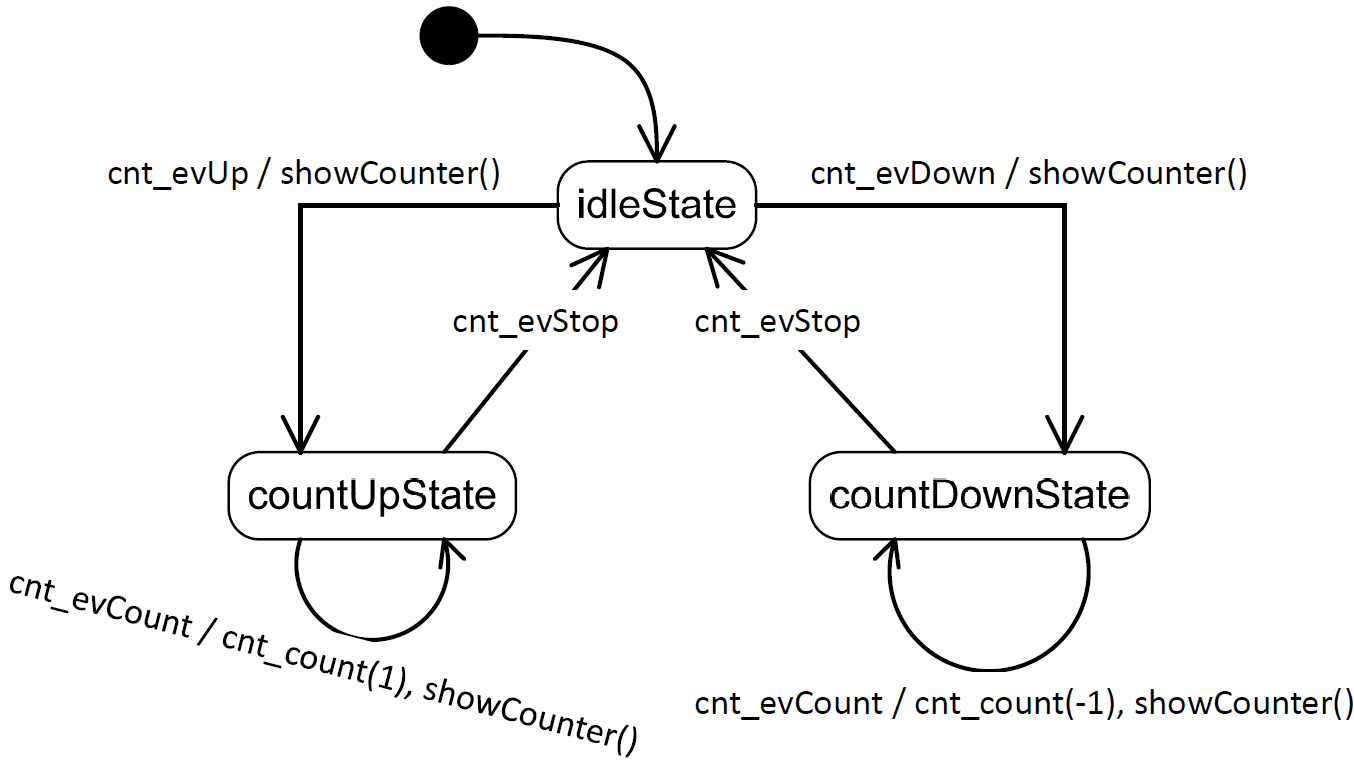
\includegraphics[width=0.7\columnwidth]{images/fsm_up-down-counter_diagramm_C.png}
\end{center}


\subsubsection{Eigenschaften der Prozeduralen Realisierung in C}






\subsection{Realisieurng mit Steuerkonstrukt (objektorientiert in C++)}

% \begin{center}
%     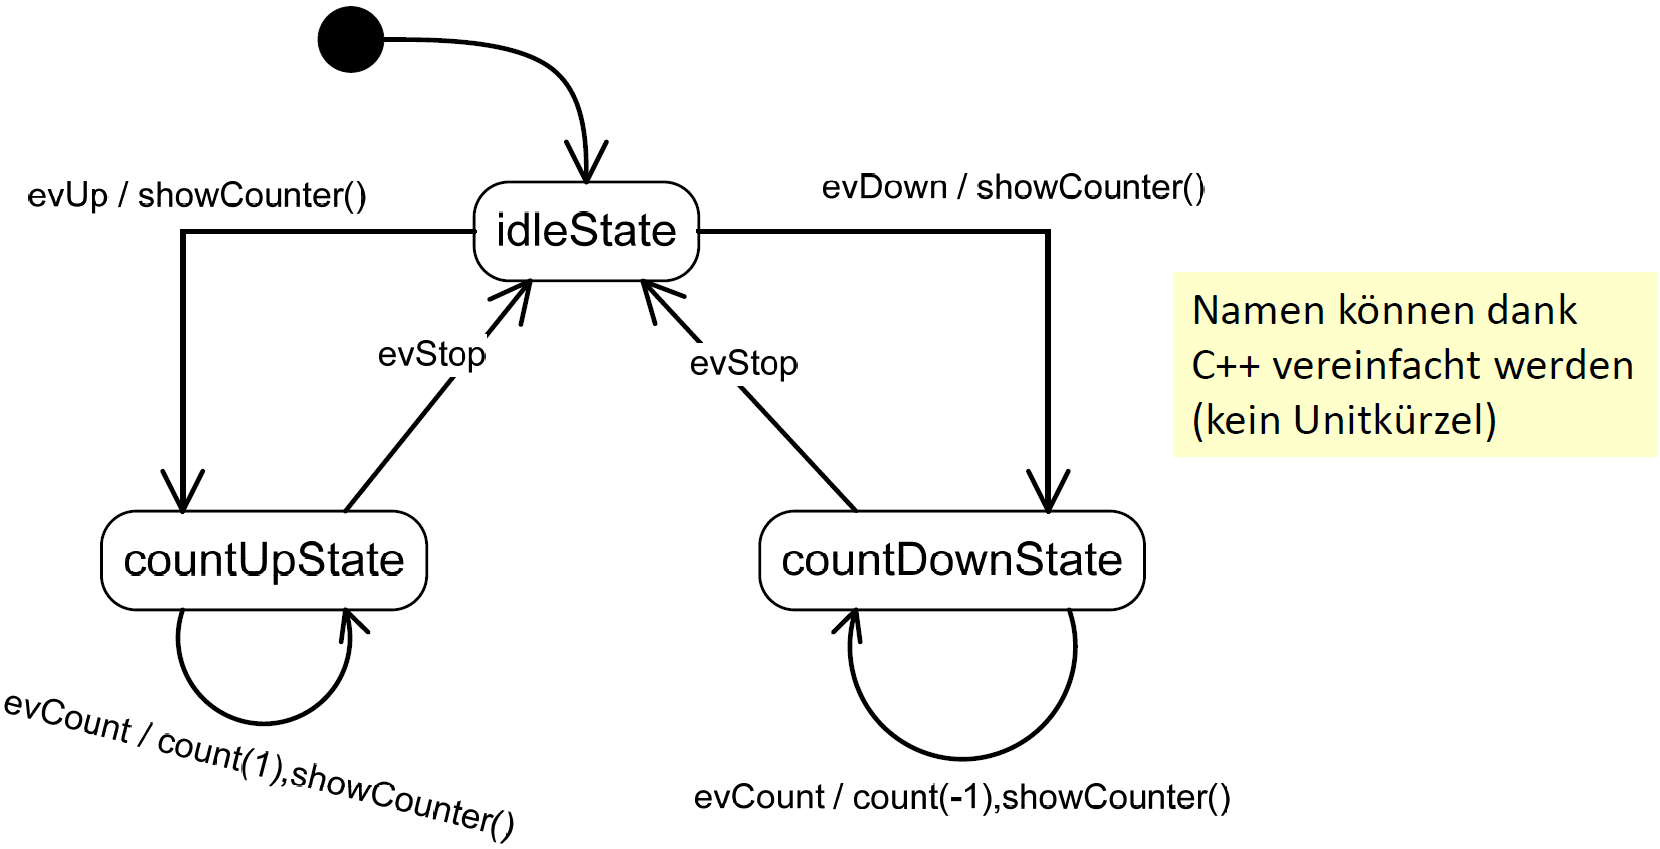
\includegraphics[width=0.7\columnwidth]{images/fsm_up-down-counter_diagramm_CPP.png}
% \end{center}


\subsection{Realisierung mit Tabelle}


\subsubsection{Performancesteigerung mit inline-Funktionen}


\subsubsection{Execution Engine}